
\documentclass[../../layout.tex]{subfiles}

\begin{document}
\chapter{Fundamentação teórica}
\hspace*{3em}O estudo, entendimento e compreensão dos conceitos abordados nesse projeto são de suma extrema importância para sua compreensão.

\section{Internet das Coisas}
\hspace*{3em}Com o desenvolvimento e demanda massiva de um mundo mais tecnológico, muitos conceitos sobre tecnologia foram surgindo e moldando a sociedade \acite{iot}. Uma dessas tecnologias em que fazemos uso é a Internet das Coisas (\emph{Internet of Things}), na qual podemos brevemente resumir em um sistema de equipamentos, dispositivos, máquinas, objetos, animais ou pessoas que possam comunicar entre si, com identificações únicas, capazaes de transferir dados através de conexões ou redes sem necessitar interação humana ou de um humano com umma máquina \cite{iot}. Exemplos reais são carros capazes de enviar sinais ao celular do motorista quando a pressão dos pneus está baixa ou monitoramento de um implante de coração pela central de um hospital, em que esses dados possam ser endereçados utilizando um protocolo de internet (IP). O objetivo principal da Internet das Coisas é poder com que essas comunicações sejam mais eficientes, rápidas,e seguras e até realizar tomadas de decisões. Um sistema em que utiliza o conceito de internet das coisas pode ser organizado em:
\begin{enumerate}[label=\alph*)]
\itemsep0em
\item coleta de dados senso gerados por sensores, pararelhos ou máquinas;
\item consolidação e envios dos dados através de uma conexão;
\item análise dos dados para realizar as ações ou tomada de decisões.
\end{enumerate}

\begin{figure}[H]
\centering
\caption{Exemplo de um sistema \emph{IoT}}
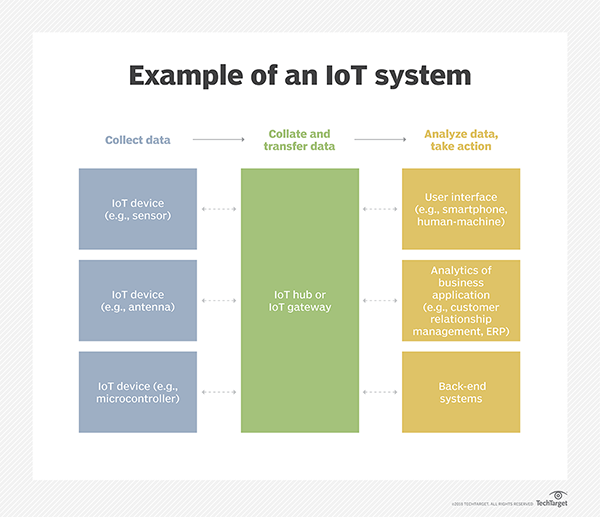
\includegraphics[width=0.5\textwidth]{assets/static/img/iot_system.jpg}
\label{fig:i2c}

\begin{minipage}{0.5\textwidth}
\raggedright \footnotesize Fonte: Retirado de \acite{iot_system} 
\end{minipage}
\end{figure}

\subsection{Evolução da Internet das Coisas}
\hspace*{3em}Na década de 90 a internet foi capaz de facilitar muitos negócios, porém era muito impactada ainda pela velocidade de conexão e dificuldade de acesso \cite{iot_evolution}. Nos anos 2000 a conectivade com a internet estava muito mais popular ao ponto de muitas aplicações estarem utilizando e que hoje dependem muito dessa tecnologia chamada internet, porém, ainda dependem da interação do ser humano ou de outras máquinas para terem algum resultado e agregarem valor, seja para acessar uma página da internet para pesquisas ou realizar negócios em um site de vendas, sendo que o maior valor está em poder realizar essas "coisas" de maneira dinâmica e automatizada, na qual podemos citar Internet das Coisas. Essa ideia é mais comum ainda nos dias atuais, pois temos várias "coisas" dentro de residências em que se comunicam de maneira automatizadas, em que muitas das vezes, podem ser até controladas via um aplicativo de celular, um navegador de internet no computador ou até mesmo uma central eletrônica.

\begin{figure}[H]
\centering
\caption{Exemplo de uma casa conectada por um sistema \emph{IoT}}
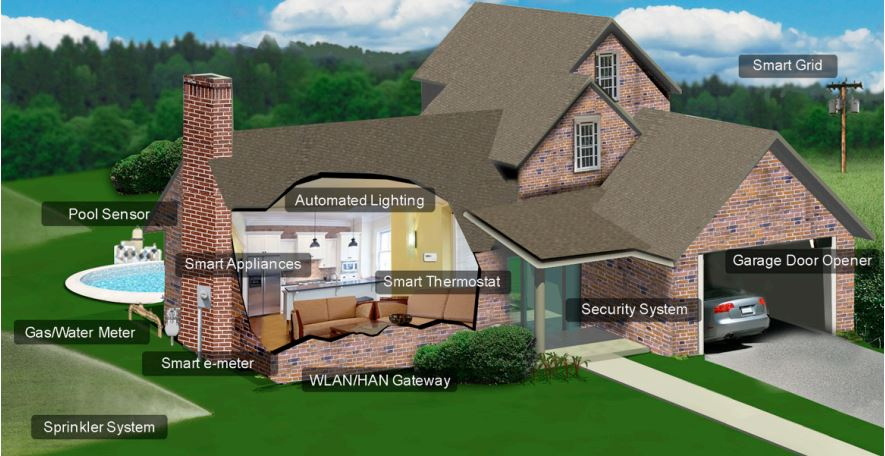
\includegraphics[width=0.5\textwidth]{assets/static/img/iothouse.jpg}
\label{fig:i2c}

\begin{minipage}{0.5\textwidth}
\raggedright \footnotesize Fonte: Retirado de \acite{iothouse} 
\end{minipage}
\end{figure}

\subsection{Indústria 4.0}
\hspace*{3em}Com a evolução da era digital, muitos setores foram impctados para ter seu melhor desempenho e crescimento. A transformação digitalização da manufatura que ocorreu durante vários anos, desde a primeira revolução industrial em que eram utilizadas máquinas à vapor, a segunda na qual utilizava eletricidade como revolução, a terceira em que faz o uso de computadores e máquinas eletrônicas até a quarta na qual tende a emergir a terceira revolução com computadores mais avançados capazes de automatizar uma linha completa com sistemas inteligentes e interligados em que o ponto principal é o tratamento de dados sendo alimentados e gerados por esses computadores \acite{ind4}.

\begin{figure}[H]
\centering
\caption{Revoluções Industriais}
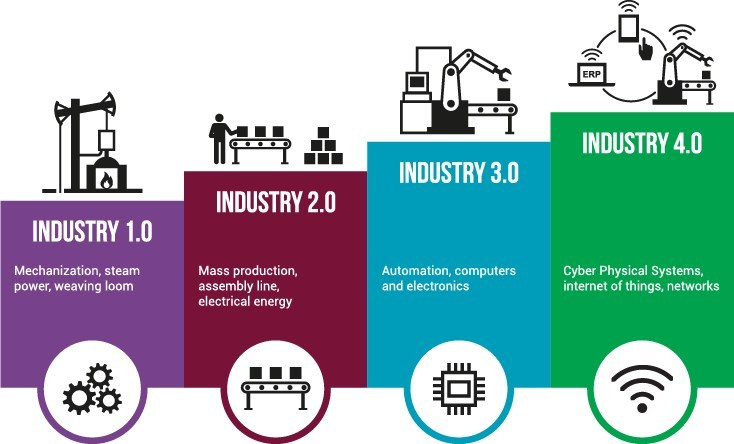
\includegraphics[width=0.5\textwidth]{assets/static/img/ind4.jpg}
\label{fig:i2c}

\begin{minipage}{0.5\textwidth}
\raggedright \footnotesize Fonte: Retirado de \acite{ind4} 
\end{minipage}
\end{figure}


\hspace*{3em}Muitos modelos de tecnologias podem ser abordados para alavancar a Indústria 4.0. Exemplos desses modelos são:
\begin{enumerate}[label=\alph*)]
\itemsep0em
    \item combinações de sistemas ciberfísicos, computacionais colaborativos que controlam entidades ou equipamentos físicos \acite{cyberphysic};
    \item internet das coisas;
    \item aprendizado de máquina (\emph{Machine Learning}).
\end{enumerate}

\hspace*{3em}Esses exemplos citados são meios utilizados para trazer valores dentro da indústria por exexmplo, para que sejam feitas análises através inúmeros dados gerados e coletados sobre performance, manutenção, rendimento, defeitos com o objetivo de identificar oportunidades, otimizar logística e a sua cadeia de gestão (\emph{Supply Chain}). Robôs inteligentes para facilitar o processo ou logística de linhas, carros autônomos para automaatizar o processo e segurança de locomoção, máquinas autônomas que possam ser totalmente independente a interação humana para executar sua função e impressão 3D são alguns dos muitos sucessos da aplicação da Indústria 4.0 no mercado atual. Apesar de parecer que estamos vivenciando essa revolução hoje em dia, estima-se que essa revolução irá permanecer em evolução durante 30 anos em que aos poucos as empresas vão adotando em seus processos.

\section{Moddelo ultilizado para aplicação}
\hspace*{3em}Para o desenvolvimento da aplicação  utilizamos o modelo cliente servidor em três camadas, esse modelo permite a modularização da aplicação  em três camadas,  camada de interface com usuário, também conhecida como front end, camada lógica onde está inserida as regras de negócio também conhecido como backend e a camada de dados  onde realiza-se a comunicação com o banco de dados, essa arquitetura permite um desacoplamento de código que viabiliza a atualização das partes de forma independente e da tecnologia \cite{3layers}
\section{REST API}
\hspace*{3em}REST (Transferência representacional de estado) API (Interface de programação de aplicação) analisando os conceitos isolados.\par
API é um interface de comunicação  disponível por software com regras estabelecidas para que haja o entendimento de ambas as partes, esse conceito vem para criar uma camada de abstração, no qual para utilizar os recursos de um determinado software é apenas necessário o entendimento da interface  disponibilizada por um software eliminado a  necessidade do entendimento total do software, além de viabilizar o conceito de modularização  de arquitetura de software.\par \cite{16}
REST é um modelo de arquitetura criado para suprir conceitos de qualidade e funcionalidade, em princípio para sistemas distribuído. Mas acabou sendo utilizada largamente em servidores WEB, a arquitetura define um conjunto de restrições para uma arquitetura estilo REST como, padrões uniformes para interfaces, sem conservação de estado e desacoplamento total do cliente e servidor, com isso permitindo a interoperabilidade entre sistemas, quando um servidor WEB segue essa restrição pode ser denominado de REST FULL.\par
Portando uma REST API é um interface que aplica os conceito REST para sua implementação\cite{19}. Quando o protocolo HTTP é utilizando o URI (Identificador de recursos uniformes) se torna uma representação dos dados e os métodos HTTP são utilizados para manipular esses dados, como o método GET para recuperar os dados, o POST para criar novos dados, PUT para atualizar os dados e DELETE para apagar os dados \cite{16}.

\section{Backend}
\subsection{Conceito de backend}
\hspace*{3em}Uma aplicação WEB em geral é dividida  em duas principais partes, a camada do front end que é responsável pela interação com o usuário de forma gráfica e o back end é responsável por entregar toda a lógica necessária para o front end, geralmente o back end é dividido em três partes, aplicação, banco de dados  e servidor, esse elementos são responsáveis por implementar a lógica do negócio \cite{16}.

\subsection{Linguagem Banckend}
\hspace*{3em}A linguagem mais utilizada para programar dispositivos IoT é a linguagem C por ser mais otimizada para essa finalidade, mas por ser uma linguagem de baixo nível, exige uma extensa dedicação de tempo e torna-se moroso para soluções mais complexas. E para contornar essas deficiências a linguagem Elixir pode ser uma ótima alternativa. Por ser uma linguagem de alto  nível que não compromete tanto a performance do sistema.\par
A linguagem Erlang/Elixir é uma linguagem funcional desenvolvida para atingir alta performance e confiabilidade. Foi desenvolvida para aplicações voltadas para telecomunicações que exigem, baixa tolerancia de falhas, distribuida e real-time (tempo de execução). Por isso conta com um conjunto bibliotecas para desenvolvimento de sistemas de alta confiabilidade conhecida como OTP.\par
Elixir foi desenvolvida para ser executada na VM (máquina virtual) do Erlang nomeada como BEAM. A linguagem Elixir é relativamente nova mas já existem diversas aplicações que a utilizam e inclusive existem recursos para dispositivo embarcado como o framework Nerves \cite{ElixirorIoT} e para implementação de aplicações WEB como o framework Phoenix.

\subsection{Nerves}
\hspace*{3em}Nerves é um framework para desenvolvimento de projetos embarcados, baseado em Linux que apenas executa a VM BEAM, portanto proporcionando a utilização da linguagem Elixir para o desenvolvimento das aplicações, dessa forma desfrutando do potencial da linguagem para implementação de projetos embarcados. Além disso este framework proporciona diversas vantagens  em relação ao processo tradicional de programação de embarcados como, permite a fácil portabilidade para diferentes HW (hardware) embarcados e com uma vasta abrangência para diferentes HW embarcados, fácil manutenção e atualização de firmware por viabilizar a atualizações via OTA (atualização sobre o ar), dispensando o processo tradicional de dispor do acesso físico a flash do dispositivo para o armazenamento do firmware, proporciona também recursos para facilitar e agilizar o desenvolvimento de firmware e uma vasta biblioteca para manipulação dos sistemas embarcados\cite{nerves}.

\subsection{Phoenix}
\hspace*{3em}Phoenix é um framework desenvolvido em Elixir para implementação de aplicações WEB, que usa todo o potencial da linguagem Elixir, com isso desfrutando da concorrência fornecida pela VM BEAM, baixa tolerância a falha e baixa latência.  Além de aumentar o desempenho do desenvolvimento de  uma aplicação WEB também conta com diversos recurso que são disponibilizados de forma modular\cite{phoenix}.

\section{Frontend}
\hspace*{3em}\blindtext[1]

\begin{figure}[H]
\centering
\caption{Diagrama do software}
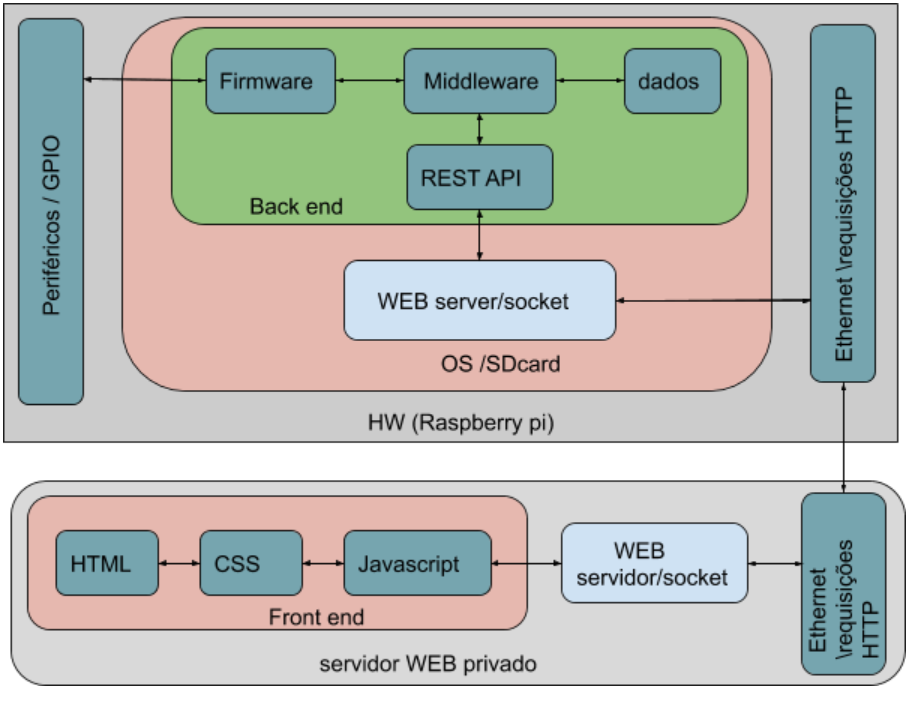
\includegraphics[width=0.5\textwidth]{assets/static/img/diagrama_tcc.PNG}
\label{fig:diagrama_sw}
\end{figure}

\section{Frameworks}
\hspace*{3em}\blindtext[1]
\subsection{Phoenix}
\hspace*{3em}\blindtext[1]
\subsection{Nerves}
\hspace*{3em}\blindtext[1]
\section{Arquivo JSON e XML}
\hspace*{3em}Para padronizar a transmissão de informações atavés da aplicações e dispositivos diferentes, foram criados vários formatos de texto para sua formatação ideal à aplicação, desenvolvedor e ao próprio usuário. Dessa forma a escolha deve ser analisada para melhor praticidade, desempenho e segurança. O formato JSON (\textit{JavaScript Object Notation}) é utilizado em aplicações compactas, de padrão aberto e de fácil compreensão , sendo muito prática para serem visualizadas de forma geral e escritas ao mesmo tempo, ao contrário de formatações como o XML (\textit{Extensible Markup Language}), O JSON é uma formatação totalmente independente que nasceu do JavaScript, porém usa convensões familiares de outras linguagens da família C(C, C++, C#), Python, Pearl, JavaScript, o que a torna muito prática para formatação em várias plataformas. A seguir, exemplos da formatação em XML e JSON:
\begin{enumerate}[label=\alph*)]
\itemsep0em
  \item XML:
    \begin{minted}[xleftmargin=\parindent,tabsize=2,breaklines]{xml}
<?xml version="1.0" encoding="UTF-8"?>
<cardapio>
<comida>
    <nome>Hot Dog</nome>
    <preco>R$ 8,99</preco>
    <descricao>
   	Pão com salsicha completo (acompanha batata palha, ketchup e maionese)
   	</descricao>
    <calorias>650</calorias>
</comida>
<comida>
    <nome>Hamburguer</nome>
    <preco>R$ 10,99</preco>
    <descricao>
    Pão com 1 fatia de hambúrguer, 3 fatias de tomate, salada, ketchup e 1 fatia de queijo
    </descricao>
    <calorias>950</calorias>
</comida>
</cardapio>
    \end{minted}
  
  \item JSON:
    \begin{minted}[xleftmargin=\parindent,tabsize=2,breaklines]{js}
[
   {
      "nome": "Hot Dog",
      "preco": "R$ 8,99",
      "descricao": "Pão com salsicha completo (acompanha batata palha, ketchup e maionese)",
      "calorias": "650"
   },
   {
      "nome": "Hamburguer",
      "preco": "R$ 10,99",
      "descricao": "Pão com 1 fatia de hambúrguer, 3 fatias de tomate, salada, ketchup e 1 fatia de queijo",
      "calorias": "950"
   }
]
    \end{minted}
\end{enumerate}

O formato JSON, como mencionado, tem um visual mais limpo, com uma leitura mais simples do arquivo e maior velocidade na manipulação e transmissão dos dados.
\section{Protocolos de comunicação}
\hspace*{3em}Com a demanda do uso de tecnologias relacionadas à área de Internet das Coisas, várias camadas de comunicação e estruturas se adaptam para maior praticidade do uso de dispositivos diversos, que por sua grande maioria se tratam de microcontroladores e sensores, na qual estão conectados entre si, seja por LAN (\emph{Local Area Network}) ou WiFi (\emph{Wireless Fidelity}). Para que essa comunicação seja eficaz e segura, foram padronizados protocolos de comunicação que são vastamente utilizados no período atual por várias empresas.

\subsection{i2c}
\hspace*{3em}O I2C é um protocolo de comunicação em que o dado é transferido \emph{bit} a \emph{bit} através de uma única conexão de uma maneira síncrona, fazendo com que a saída desse sinal seja baseada no clock (\emph{período de oscilação}) enviado do \emph{Master} (Mestre) ao \emph{Slave} (Escravo), onde esse clock é apenas dependente do Master. Esse método de comunicação necessita apenas de 2 conexões, o SDA (\emph{Serial Data Access}) e o SCL (\emph{Serial Clock Access}).

\begin{figure}[H]
\centering
\caption{Protocolo I2C}
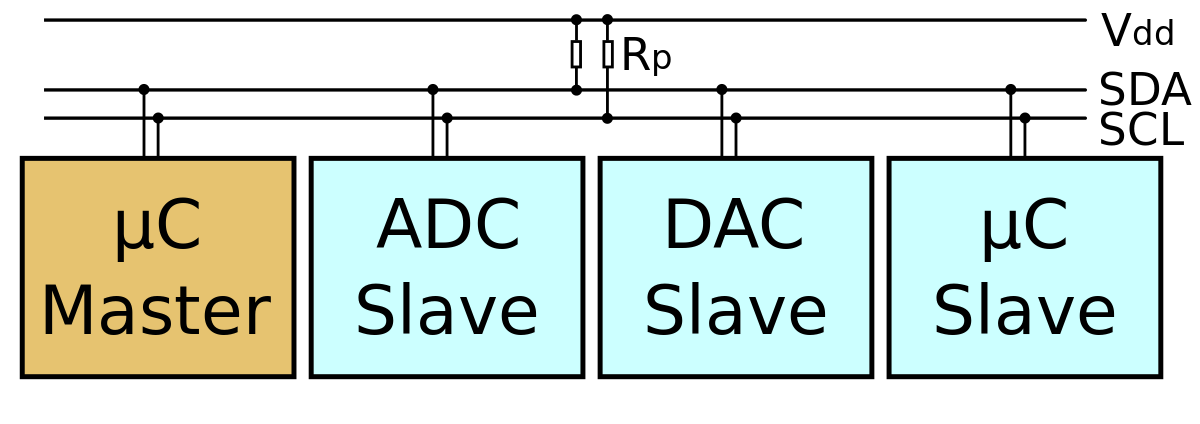
\includegraphics[width=0.5\textwidth]{assets/static/img/i2c.jpg}
\label{fig:i2c}

\begin{minipage}{0.5\textwidth}
\raggedright \footnotesize Fonte: Retirado de \acite{i2c} 
\end{minipage}
\end{figure}

\hspace*{3em}Com a comunicação via I2C, os dados são quebrados em pequenos pacotes em que formam esse padrão. Esses pacotes contém informações do endereço do \emph{Slave}, \emph{bits} de condição de início e fim da menssagem transmitida, o dado a ser transmitido e um sinal de \emph{feedback} chamado de positivo ACK (\emph{Acknowledge bit}) quando a mensagem é entregue ao escravo, ou negativo NACK (\emph{No-acknowledge bit}) quando a mensagem não é entregue ao escravo, de acordo com a figura \ref{fig:i2c_structure}.

\begin{figure}[H]
\centering
\caption{i2c_structure}
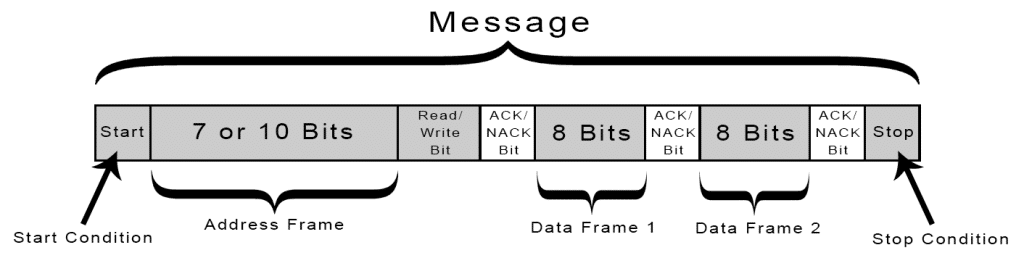
\includegraphics[width=0.5\textwidth]{assets/static/img/i2c_structure.jpg}
\label{fig:i2c_structure}

\begin{minipage}{0.5\textwidth}
\raggedright \footnotesize Fonte: Retirado de \cite{i2c_structure} 
\end{minipage}
\end{figure}

\subsection{UART}
\hspace*{3em}A comunicação UART (\emph{Universal Asynchronous Receiver-Transmitter}) é um dispositiivo presente dentro de um microcontrolador em que seu objetivo é controlar a entrada e saída de dados através de sequências de 8 \emph{bits}. Atualmente é o método mais comum para comunicação serial \emph{full-duplex} \cite{uart} A comunicação UART não se refere apenas à um protocolo, mas um conjuto completo de circuitos integrados. Os dispositivos UART possuem duas conexões, uma para transmitir dados (TX) e outra para receber os dados (RX), de uma maneira totalmente assíncrona ao \emph{clock}. Da mesma forma que citamos do I2C, o UART também utiliza \emph{bits} para identificação do início e fim do pacote enviado ou recebido. Importante citar que todos os dispositivos no circuito devem ter o mesmo \emph{baud rate} (taxa de transmissão) como padronização.

\chapter{Modelagem do Hardware}
\hspace*{3em}A montagem e relação entre os dispositivos, microcontroladores e conexões pode ser resumida de acordo com a seguinte exemplicifação: o microcomputador comunica ou com os sensores e dispositivos, sejam eles sensores de temperatura, humidade, luminosidade que camptam valores do ambiente em que se localiza ou com lâmpadas ou leds e enviam para esse microcomputador, na qual é o próprio servidor em que armazena localmente suas informações recebidas e processa de forma organizada para otimizar seu uso. Esse microcomputador processa então essas informações para representar como interface humana para que o usuário possa integarir, através de um navegador da internet em outro aparelho qualquer, seja celular ou computador. Na Figura \ref{fig:hwmodel} é representado o diagrama de blocos do hardware deste projeto, onde são separadas por 3 partes principais:

\begin{enumerate}[label=\alph*)]
\itemsep0em
    \item Fonte de alimentação; 
    \item Raspberry Pi 3 B+, o microcomputador do projeto;
    \item Sensores, responsáveis pela comunicação externa do microcomputador ao ambiente instalado.
\end{enumerate}
 
\begin{figure}[H]
\centering
\caption{Diagrama de \emph{Hardware}}
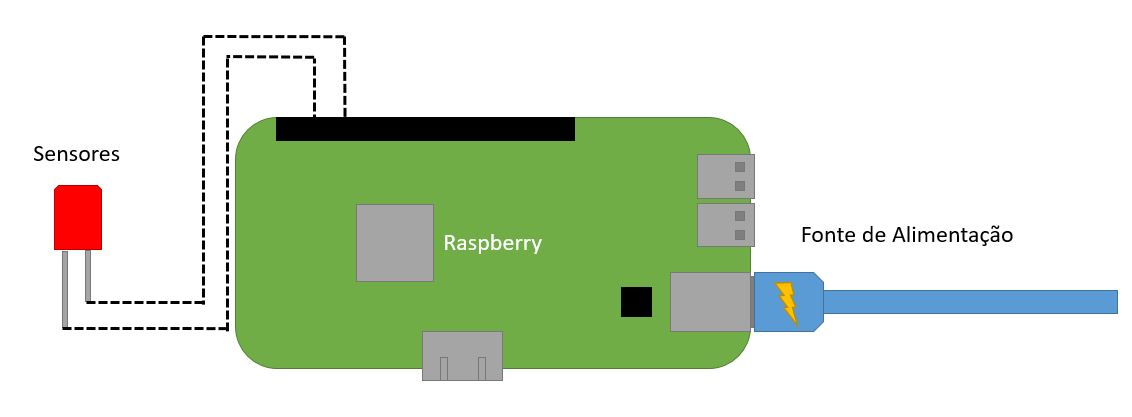
\includegraphics[width=0.5\textwidth]{assets/static/img/hwmodel.jpg}
\label{fig:i2c_structure}

\begin{minipage}{0.5\textwidth}
\raggedright \footnotesize Fonte: autor 
\end{minipage}
\end{figure}

\hspace*{3em}Neste projeto foi escolhido o microcomputador Raspberry Pi 3 B+, exibido na Figura \ref{fig:rpi}, desenvolvido no final de 2014 pela \emph{Raspberry Pi Foundation} com as seguintes especificações:
\begin{enumerate}[label=\alph*)]
\itemsep0em
    \item SoC (\emph{System On a Chip}): Broadcom BCM2837B0 quad-core Cortex-A53 (ARMv8) 64-bit 1.4GHz;
    \item 1 entrada \emph{Gigabit Ethernet} e WiFi (2,4 e 5 GHz);
    \item memória: 1GB LPDDR2 SDRAM;
    \item GPIO (\emph{General Purpose Input/Output})de 40 pinos;
    \item Entrada de 5V/ 2,5A;
    \item memória: 1GB LPDDR2 SDRAM;
    \item armazenamento: cartão \emp{Micro SD}.
\end{enumerate}

\begin{figure}[H]
\centering
\caption{Raspberry Pi}
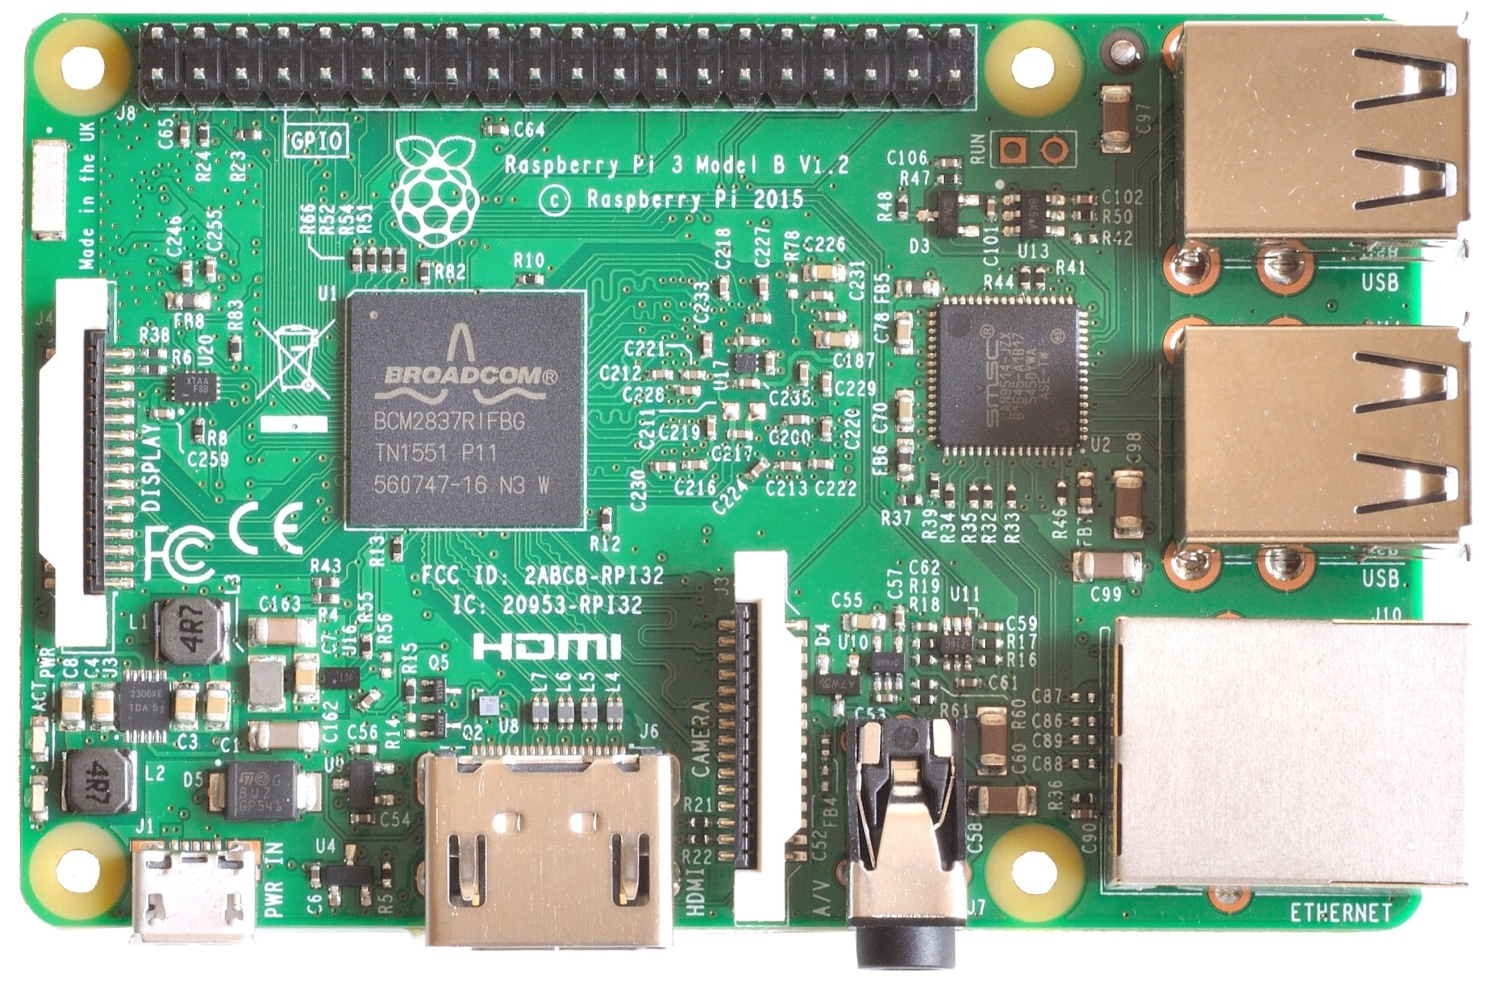
\includegraphics[width=0.5\textwidth]{assets/static/img/rpi.jpg}
\label{fig:rpi}

\begin{minipage}{0.5\textwidth}
\raggedright \footnotesize Fonte: Retirado de \acite{rpi}
\end{minipage}
\end{figure}

\hspace*{3em}O motivo deste microprocessador ser escolhido foi devido à praticidade de seu uso, seja informações na internet, quanto a portabilidade nas conexões de GPIO, conexão à internet via cabo ou WiFi, quantidade de memória suficiente para um sistema operacional ideal, baixo consumo de energia e preço agressivo comparado à outros modelos de processadores ou microprocessadores.

\section{Sensores}
\section{Conexão dos sensores à Raspberry Pi 3B+}
\hspace*{3em}Todas as conexões que realizamos dos sensores e leds foram feitas atráves da GPIO do microprocessador, o Raspberry, através de uma \emph{protoboard} e cabos para conectá-los.
\hspace*{3em}Sensores, atuadores, microcontroladores são componentes vastamente utilizados para projetos de Internet das Coisas para sua conectividade e interação sejam realizadas \cite{sensores_iot}. Sensores por sua vez, são prático e de baixo custo para trazer um valor final ao projeto, como monitorar temperatura de uma sala de servidor, controlar humidade de um campo de plantações, abertura de cortinas de plantações, entre outros objetivos.
\subsection{Sensor de Luminosidade - BH1750}
\hspace*{3em}O sensor de luminosidade BH1750 é um dispositivo sensível à luz que possui uma interface de comunicação 16 \emph{bits} e interface de comunicação de acordo com o protocolo I2C e uma característica de sensibilidade ao espectro de luz muito parecido ao olho humano.
\hspace*{3em}O sensor BH1750 possui as seguintes especificações:
\begin{enumerate}[label=\alph*)]
\itemsep0em
    \item sensor de luminosidade com faixa de operação de 1 lux a 65.535 lux, precisão de +/- 1 lux e resolução de 1 lux.
\end{enumerate}

\begin{figure}[H]
\centering
\caption{Sensor de Luminosidade - BH1750}
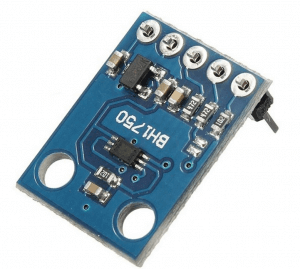
\includegraphics[width=0.5\textwidth]{assets/static/img/BH1750.jpg}
\label{fig:BH1750}

\begin{minipage}{0.5\textwidth}
\raggedright \footnotesize Fonte: Retirado de \cite{BH1750} 
\end{minipage}
\end{figure}

\hspace*{3em}Esse dispositivo tem configuração de  Entrada e Saída para 5 pinos, sendo eles: alimentação (Vcc e Terra), pinos para o protocolo I2C (SCL e SDA) e um pino analógico para o valor do sensor, nomeado como ADDR.

\begin{figure}[H]
\centering
\caption{Pinos BH1750}
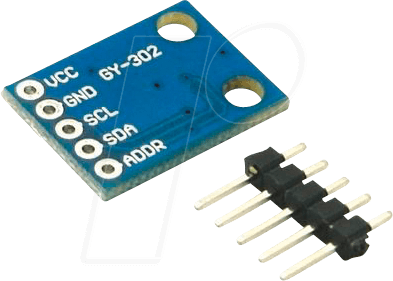
\includegraphics[width=0.5\textwidth]{assets/static/img/BH1750_pinout.jpg}
\label{fig:BH1750_pinout}

\begin{minipage}{0.5\textwidth}
\raggedright \footnotesize Fonte: Retirado de \cite{BH1750_shop} 
\end{minipage}
\end{figure}

\subsection{Sensor de Temperatura e Humidade - dht11}
\hspace*{3em}O sensor dht11 é um dispositivo sensível à temperatura e humidade que pode ser utilizado em conjunto com vários microcontroladores, através do sensor capacitivo de umidade e um termistor para medir o ar e enviar um sinal no pino de saída do mesmo. O sensor dht11 possui as seguintes especificações:
\begin{enumerate}[label=\alph*)]
\itemsep0em
    \item sensor de temperatura com faixa de operação de 0ºC a 50ºC, precisão de +/- 2ºC e resolução de 1ºC;
    \item sensor de humidade com faixa de operação de 20\%HR a 90\%HR, precisão de +/- 5\%HR e resolução de 1\%HR.
\end{enumerate}

\begin{figure}[H]
\centering
\caption{Pinos dht11}
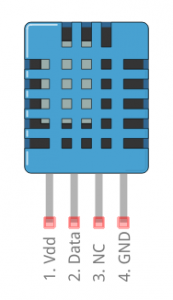
\includegraphics[width=0.5\textwidth]{assets/static/img/dht11_pinout.jpg}
\label{fig:BH1750_pinout}

\begin{minipage}{0.5\textwidth}
\raggedright \footnotesize Fonte: Retirado de \cite{dht11_pinout} 
\end{minipage}
\end{figure}

\hspace*{3em}A comunicação que é mais utilizada para esse dispositivo é a \emph{adhoc} dh11. 

\chapter{Estrutura do Software}
\hspace*{3em}\blindtext[1]
\chapter{Método}
\hspace*{3em}\blindtext[1]
\end{document}
